% Detailed layer-level architecture of the Stage-2 MeanFlow residual head
% MF_theta (MeanFlowPrecond, trained). All module names, channel transitions
% and parameter counts are measured by instantiating the canonical 192x96
% network (stormcast/meanflow_architecture.md, "Full layer inventory").
% Symbols follow the meancasthd.png schematic: M_t, mu_{t+1}, I, MF_theta.
\documentclass[border=12pt]{standalone}
% Shared style for the MeanFlow thesis figures.
% Clean academic grayscale, in the spirit of the nntikz examples
% (rounded gray!10 blocks, -latex arrows). Self-contained: this does NOT
% depend on the legacy presentation/meanflow_workflow/src/mf_style.tex.
\usepackage{amsmath,amssymb,bm}
\usepackage{tikz}
\usetikzlibrary{positioning,arrows.meta,calc,fit,backgrounds,shapes.geometric,chains,decorations.pathmorphing}

\tikzset{
  % --- generic nodes ---------------------------------------------------
  base/.style    ={rounded corners=2.5pt, draw, line width=0.8pt, align=center,
                   inner sep=5pt, font=\small, text=black!88},
  block/.style   ={base, fill=gray!10},
  data/.style    ={base, fill=white},                       % data / tensors
  net/.style     ={base, fill=gray!22, line width=1.0pt},   % trained network
  frozen/.style  ={base, fill=gray!4, draw=black!60,        % frozen network
                   dash pattern=on 3pt off 2pt},
  loss/.style    ={base, fill=gray!10, line width=1.0pt,    % loss / scalar
                   double, double distance=1.2pt},
  emph/.style    ={base, fill=gray!10, line width=1.3pt},   % highlighted box
  % --- operator glyphs -------------------------------------------------
  op/.style      ={circle, draw, line width=0.8pt, fill=white,
                   minimum size=4.6mm, inner sep=0, font=\footnotesize},
  concat/.style  ={rectangle, rounded corners=1pt, draw, fill=black!72,
                   text=white, font=\scriptsize\bfseries, inner sep=2.5pt},
  % --- arrows ----------------------------------------------------------
  arrow/.style   ={-{Latex[length=2.4mm]}, line width=0.8pt, draw=black!82},
  arrowc/.style  ={arrow, rounded corners=3pt},
  thinarrow/.style={-{Latex[length=2.0mm]}, line width=0.6pt, draw=black!55},
  loopback/.style={-{Latex[length=2.4mm]}, line width=0.8pt, draw=black!55,
                   dashed, dash pattern=on 4pt off 3pt},
  % --- containers / annotation ----------------------------------------
  group/.style   ={rounded corners=5pt, draw=black!40, line width=0.7pt,
                   dashed, dash pattern=on 3pt off 2.5pt, fill=black!2,
                   inner sep=8pt},
  ttl/.style     ={font=\bfseries\large, text=black!88},
  sub/.style     ={font=\itshape\footnotesize, text=black!55},
  lab/.style     ={font=\scriptsize, text=black!70},
  tag/.style     ={font=\scriptsize\bfseries, text=black!60},
  % small sine glyph used to mark Fourier / positional embeddings
  sinewave/.style={decorate, decoration={snake, amplitude=0.6mm,
                   segment length=2.2mm}},
}

% legend swatch helper: \swatch{<style>}{<label>}
\newcommand{\swatch}[2]{%
  \tikz[baseline=-0.5ex]\node[#1, minimum width=3.6mm, minimum height=2.8mm,
    inner sep=0]{};\;#2}

\begin{document}
\newcommand{\restag}[1]{{\tiny\bfseries\textcolor{black!55}{#1}}}
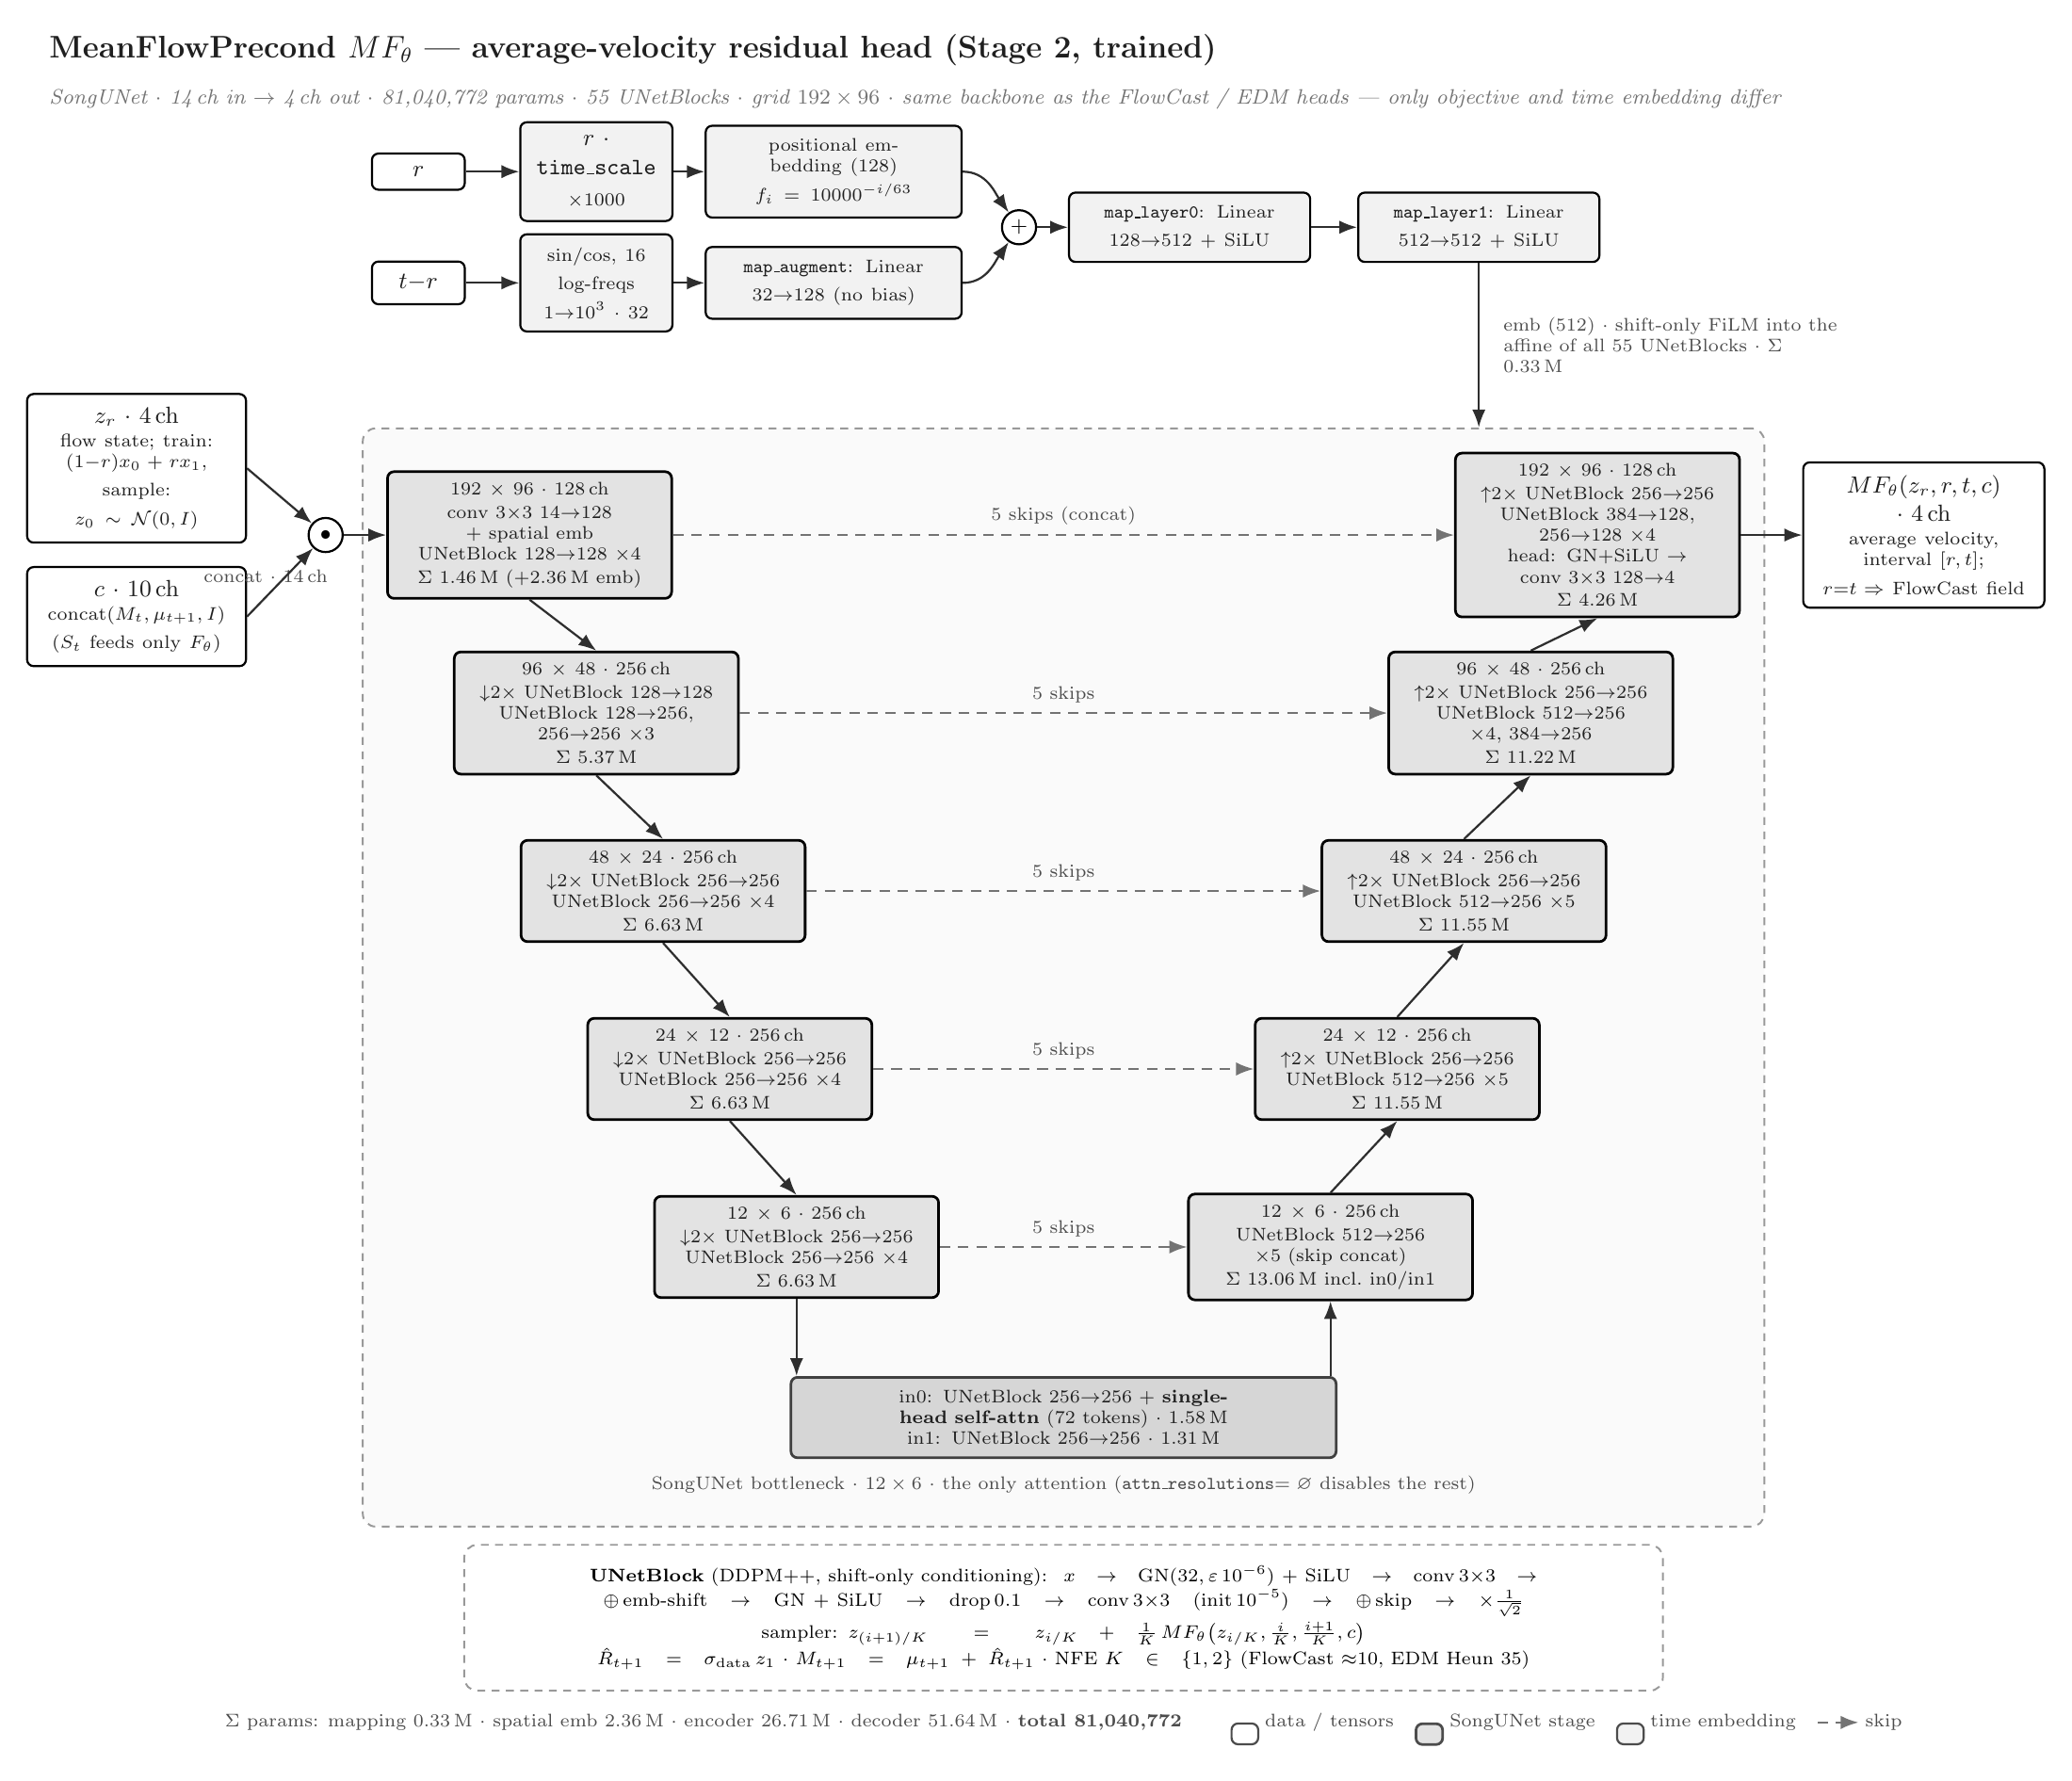
\begin{tikzpicture}
  \tikzset{ustage/.style={net, text width=3.55cm, font=\scriptsize, inner sep=4pt}}

  % ============================ inputs + concat ============================
  \node[data, text width=2.6cm] (zr) at (-5.3, 0.9)
    {$z_r$ $\cdot$ 4\,ch\\[1pt]\scriptsize flow state; train:
     $(1{-}r)x_0 + r x_1$,\\\scriptsize sample: $z_0 \sim \mathcal{N}(0, I)$};
  \node[data, text width=2.6cm] (ct) at (-5.3,-1.1)
    {$c$ $\cdot$ 10\,ch\\[1pt]\scriptsize $\mathrm{concat}(M_t, \mu_{t+1}, I)$\\
     \scriptsize ($S_t$ feeds only $F_\theta$)};
  \node[op] (cc) at (-2.75, 0) {$\bullet$};
  \node[lab, anchor=north east] at ($(cc.south)+(1.5mm,-1mm)$) {concat $\cdot$ 14\,ch};

  \draw[arrow] (zr.east) -- (cc);
  \draw[arrow] (ct.east) -- (cc);

  % ============================ encoder (staircase down-right) ============================
  \node[ustage] (e0) at (0.0, 0.0) {%
    \restag{$192\times96$ $\cdot$ 128\,ch}\\[1pt]
    conv $3{\times}3$ $14{\to}128$ $+$ spatial emb\\
    UNetBlock $128{\to}128$ $\times4$\\[1pt]
    $\Sigma$ 1.46\,M ($+$2.36\,M emb)};
  \node[ustage] (e1) at (0.9,-2.4) {%
    \restag{$96\times48$ $\cdot$ 256\,ch}\\[1pt]
    ${\downarrow}2{\times}$ UNetBlock $128{\to}128$\\
    UNetBlock $128{\to}256$, $256{\to}256$ $\times3$\\[1pt]
    $\Sigma$ 5.37\,M};
  \node[ustage] (e2) at (1.8,-4.8) {%
    \restag{$48\times24$ $\cdot$ 256\,ch}\\[1pt]
    ${\downarrow}2{\times}$ UNetBlock $256{\to}256$\\
    UNetBlock $256{\to}256$ $\times4$\\[1pt]
    $\Sigma$ 6.63\,M};
  \node[ustage] (e3) at (2.7,-7.2) {%
    \restag{$24\times12$ $\cdot$ 256\,ch}\\[1pt]
    ${\downarrow}2{\times}$ UNetBlock $256{\to}256$\\
    UNetBlock $256{\to}256$ $\times4$\\[1pt]
    $\Sigma$ 6.63\,M};
  \node[ustage] (e4) at (3.6,-9.6) {%
    \restag{$12\times6$ $\cdot$ 256\,ch}\\[1pt]
    ${\downarrow}2{\times}$ UNetBlock $256{\to}256$\\
    UNetBlock $256{\to}256$ $\times4$\\[1pt]
    $\Sigma$ 6.63\,M};

  % ============================ decoder (staircase up-right) ============================
  \node[ustage] (d4) at (10.8,-9.6) {%
    \restag{$12\times6$ $\cdot$ 256\,ch}\\[1pt]
    UNetBlock $512{\to}256$ $\times5$ (skip concat)\\[1pt]
    $\Sigma$ 13.06\,M incl.\ in0/in1};
  \node[ustage] (d3) at (11.7,-7.2) {%
    \restag{$24\times12$ $\cdot$ 256\,ch}\\[1pt]
    ${\uparrow}2{\times}$ UNetBlock $256{\to}256$\\
    UNetBlock $512{\to}256$ $\times5$\\[1pt]
    $\Sigma$ 11.55\,M};
  \node[ustage] (d2) at (12.6,-4.8) {%
    \restag{$48\times24$ $\cdot$ 256\,ch}\\[1pt]
    ${\uparrow}2{\times}$ UNetBlock $256{\to}256$\\
    UNetBlock $512{\to}256$ $\times5$\\[1pt]
    $\Sigma$ 11.55\,M};
  \node[ustage] (d1) at (13.5,-2.4) {%
    \restag{$96\times48$ $\cdot$ 256\,ch}\\[1pt]
    ${\uparrow}2{\times}$ UNetBlock $256{\to}256$\\
    UNetBlock $512{\to}256$ $\times4$, $384{\to}256$\\[1pt]
    $\Sigma$ 11.22\,M};
  \node[ustage] (d0) at (14.4, 0.0) {%
    \restag{$192\times96$ $\cdot$ 128\,ch}\\[1pt]
    ${\uparrow}2{\times}$ UNetBlock $256{\to}256$\\
    UNetBlock $384{\to}128$, $256{\to}128$ $\times4$\\
    head: GN$+$SiLU $\to$ conv $3{\times}3$ $128{\to}4$\\[1pt]
    $\Sigma$ 4.26\,M};

  % ============================ bottleneck ============================
  \node[net, fill=gray!32, draw=black!75, text width=7.0cm, font=\scriptsize]
    (bk) at (7.2,-11.9)
    {in0: UNetBlock $256{\to}256$ $+$ \textbf{single-head self-attn} (72 tokens) $\cdot$ 1.58\,M\\
     in1: UNetBlock $256{\to}256$ $\cdot$ 1.31\,M};
  \node[lab, anchor=north] (bkcap) at ($(bk.south)+(0,-1mm)$)
    {SongUNet bottleneck $\cdot$ $12\times6$ $\cdot$ the only attention
     (\texttt{attn\_resolutions}$=\varnothing$ disables the rest)};

  % ============================ U-Net container ============================
  \begin{scope}[on background layer]
    \node[group, fit=(e0)(e4)(bk)(bkcap)(d4)(d0), inner sep=9pt] (unet) {};
  \end{scope}

  % ============================ main data path ============================
  \draw[arrow] (cc) -- (e0.west);
  \draw[arrow] (e0.south) -- (e1.north);
  \draw[arrow] (e1.south) -- (e2.north);
  \draw[arrow] (e2.south) -- (e3.north);
  \draw[arrow] (e3.south) -- (e4.north);
  \draw[arrow] (e4.south) -- ($(bk.north -| e4.south)$);
  \draw[arrow] ($(bk.north -| d4.south)$) -- (d4.south);
  \draw[arrow] (d4.north) -- (d3.south);
  \draw[arrow] (d3.north) -- (d2.south);
  \draw[arrow] (d2.north) -- (d1.south);
  \draw[arrow] (d1.north) -- (d0.south);

  % ============================ skip connections ============================
  \draw[loopback] (e0.east) -- node[lab,above,pos=0.5]{5 skips (concat)} (d0.west);
  \draw[loopback] (e1.east) -- node[lab,above,pos=0.5]{5 skips} (d1.west);
  \draw[loopback] (e2.east) -- node[lab,above,pos=0.5]{5 skips} (d2.west);
  \draw[loopback] (e3.east) -- node[lab,above,pos=0.5]{5 skips} (d3.west);
  \draw[loopback] (e4.east) -- node[lab,above,pos=0.5]{5 skips} (d4.west);

  % ============================ output ============================
  \node[data, text width=2.9cm] (out) at (18.8, 0.0)
    {$MF_\theta(z_r, r, t, c)$ $\cdot$ 4\,ch\\[1pt]
     \scriptsize average velocity,\\
     \scriptsize interval $[r,t]$;\\
     \scriptsize $r{=}t \Rightarrow$ FlowCast field};
  \draw[arrow] (d0.east) -- (out.west);

  % ============================ time-conditioning rails (MeanFlow-specific) ============================
  \node[data, text width=0.9cm]  (r)    at (-1.5, 4.9) {$r$};
  \node[block, text width=1.7cm] (rsc)  at (0.9, 4.9)
    {$r \cdot \texttt{time\_scale}$\\[1pt]\scriptsize $\times 1000$};
  \node[block, text width=3.1cm] (remb) at (4.1, 4.9)
    {\scriptsize positional embedding (128)\\$f_i = 10000^{-i/63}$};
  \node[data, text width=0.9cm]  (gap)  at (-1.5, 3.4) {$t{-}r$};
  \node[block, text width=1.7cm] (four) at (0.9, 3.4)
    {\scriptsize sin/cos, 16 log-freqs $1{\to}10^{3}$ $\cdot$ 32};
  \node[block, text width=3.1cm] (aug)  at (4.1, 3.4)
    {\scriptsize \texttt{map\_augment}: Linear $32{\to}128$ (no bias)};
  \node[op] (opm) at (6.6, 4.15) {$+$};
  \node[block, text width=2.9cm] (ml0) at (8.9, 4.15)
    {\scriptsize \texttt{map\_layer0}: Linear $128{\to}512$ $+$ SiLU};
  \node[block, text width=2.9cm] (ml1) at (12.8, 4.15)
    {\scriptsize \texttt{map\_layer1}: Linear $512{\to}512$ $+$ SiLU};

  \draw[arrow] (r.east)    -- (rsc.west);
  \draw[arrow] (rsc.east)  -- (remb.west);
  \draw[arrow] (gap.east)  -- (four.west);
  \draw[arrow] (four.east) -- (aug.west);
  \draw[arrow] (remb.east) to[out=0,in=125] (opm);
  \draw[arrow] (aug.east)  to[out=0,in=-125] (opm);
  \draw[arrow] (opm) -- (ml0.west);
  \draw[arrow] (ml0.east) -- (ml1.west);
  \draw[arrow] (ml1.south) -- (ml1.south |- unet.north)
    node[lab, anchor=west, pos=0.5, xshift=2mm, text width=4.6cm,
         align=left]
    {emb (512) $\cdot$ shift-only FiLM into the\\
     affine of all 55 UNetBlocks $\cdot$ $\Sigma$ 0.33\,M};

  % ============================ title ============================
  \node[ttl, anchor=south west] (title) at (-6.6, 6.2)
    {MeanFlowPrecond $MF_\theta$ --- average-velocity residual head (Stage 2, trained)};
  \node[sub, anchor=north west] at ($(title.south west)+(0,-0.6mm)$)
    {SongUNet $\cdot$ 14\,ch in $\to$ 4\,ch out $\cdot$ 81{,}040{,}772 params
     $\cdot$ 55 UNetBlocks $\cdot$ grid $192\times96$ $\cdot$ same backbone as
     the FlowCast / EDM heads --- only objective and time embedding differ};

  % ============================ UNetBlock anatomy + sampler + totals ============================
  \node[group, text width=15.6cm, font=\scriptsize, align=center, fill=white]
    (anatomy) at (7.2,-14.6)
    {\textbf{UNetBlock} (DDPM++, shift-only conditioning):\;
     $x \to \mathrm{GN}(32,\varepsilon\,10^{-6})\!+\!\mathrm{SiLU}
     \to \mathrm{conv}\,3{\times}3 \to \oplus\,\text{emb-shift}
     \to \mathrm{GN}\!+\!\mathrm{SiLU} \to \mathrm{drop}\,0.1
     \to \mathrm{conv}\,3{\times}3\;(\text{init}\,10^{-5})
     \to \oplus\,\text{skip} \to \times\tfrac{1}{\sqrt{2}}$\\[1pt]
     sampler: $z_{(i+1)/K} = z_{i/K} + \tfrac{1}{K}\,
     MF_\theta\bigl(z_{i/K}, \tfrac{i}{K}, \tfrac{i+1}{K}, c\bigr)$\\
     $\hat{R}_{t+1} = \sigma_{\text{data}}\, z_{1}$
     $\cdot$ $M_{t+1} = \mu_{t+1} + \hat{R}_{t+1}$
     $\cdot$ NFE $K \in \{1,2\}$ (FlowCast ${\approx}10$, EDM Heun $35$)};
  \node[lab, anchor=north] at ($(anatomy.south)+(0,-1.6mm)$)
    {$\Sigma$ params: mapping 0.33\,M $\cdot$ spatial emb 2.36\,M $\cdot$
     encoder 26.71\,M $\cdot$ decoder 51.64\,M $\cdot$
     \textbf{total 81{,}040{,}772} \qquad
     \swatch{data}{data / tensors}\quad
     \swatch{net}{SongUNet stage}\quad
     \swatch{block}{time embedding}\quad
     \tikz[baseline=-0.5ex]\draw[loopback](0,0)--(0.55,0);\;skip};

\end{tikzpicture}
\end{document}
